
\section{Entwicklung einer Handlungsempfehlung}
\label{sec:Handlungsempfehlung}
In einem wettbewerbsintensiven Umfeld reicht es häufig nicht aus die Bedürfnisse der Anwender zu verstehen und innovative IT-Services zu entwickeln. Stattdessen sollten Unternehmen eine höhere Priorität darauf legen, Dienste im Vergleich zur Konkurrenz schneller bereitzustellen. Infolgedessen verwenden 62 Prozent aller Unternehmensentwickler CI/CD-Tools innerhalb ihrer Bereitstellungsprozesse. Die kontinuierliche Integration und Bereitstellung von Software bietet dabei insbesondere für CEs erhebliche Vorteile. Obwohl einzelne Module einer CEA grundsätzlich isoliert voneinander betrieben werden, können Abhängigkeiten zwischen diesen entstehen. Im Kontext eines Composable-ERP-Systems könnte es etwa erforderlich sein, dass die in einem Vertriebsmodul abgewickelten Verkäufe in das Finanzwesen übertragen werden müssen. Insbesondere bei der Zusammenarbeit vieler Entwickler kann diese Integration zu erheblichem Koordinationsaufwand führen. Wenn Teams nicht in der Lage sind effektiv miteinander zu kommunizieren, besteht das Risiko, dass Konflikte in der gemeinsamen Code-Basis entstehen. Um dieser Herausforderung zu begegnen, bietet sich die Implementierung einer CI/CD-Pipeline. Dabei wird der lokale Quell-Code der Entwickler kontinuierlich und automatisiert mit dem Hauptzweig des Repositories zusammengeführt und mit dem bestehenden Code getestet. Statt Code-Reviews und Validierungen erst in einer späten Phase des Softwareerstellungszykluses abzuwickeln (\textit{Shift-Right}), werden Tests bereits während der Entwicklung durchgeführt (\textit{Shift-Left}). Nach Erstellung einer Funktionalität bekommen Entwickler über verschiedene Kommunikationskanäle (z.B. E-Mail) unmittelbares Feedback und können den Service somit optimieren, bis dieser den Produktstandards des Unternehmens entspricht. Dieser Ansatz zielt darauf ab, eine frühzeitige Identifikation und Behebung von Fehlern zu erleichtern. Darüber hinaus ermöglichen CI/CD-Pipelines den Aufbau standardisierter Testinfrastrukturen. Damit können neue Features automatisiert in Systemumgebungen getestet werden, bei welchen Betriebssysteme, Systembibliotheken, Abhängigkeiten und Konfigurationseinstellungen an die Produktion angepasst sind. Zum einen können somit potenzielle Fehler erkannt werden, welche ansonsten im produktiven Betrieb auftreten würden.  Darüber hinaus entfällt durch das automatische Abwickeln dieser Prozesse, ebenfalls ein manuelles Aufsetzen der Testinfrastruktur. So können CEs ihre Ressourcen vermehrt auf das Kerngeschäft, also die Entwicklung neuer ERP-Funktionalitäten, konzentrieren. Da für jeden Microservice i.d.R. eine CI- sowie CD-Pipeline betrieben wird, gestaltet es sich insbesondere bei einer umfassenden CEA als herausfordernd, den gesamten Bereitstellungsprozess zu überwachen. Dabei Abhilfe schaffen sollen Monitoring-Dashboards, mit welchen die gesamten Pipeline-Workflows eines ERP-Systems in einem zentralen Tool überwacht werden können. Die dabei analysierten Metriken werden ebenfalls in einen historischen Datenkontext eingeordnet, womit Entwickler-Teams Trends in der Code-Qualität identifizieren können. Dies ermöglicht eine Ermittlung von Muster in vorliegenden Fehlerdaten, womit Problembereiche der bestehenden Code-Basis erkannt und deren Korrektur priorisiert werden kann. Der von Panorama Consulting Solutions veröffentlichte ERP Report 2019 zeigt, dass ERP-Systeme aufgrund der Geschwindigkeit mit welcher sich Unternehmenstechnologien und Marktdynamiken entwickeln, zukunftsorientiert sein müssen \cite{.c}. Statt auf wiederholte kostspielige Migrationen zurückgreifen zu müssen, sollten Unternehmen daher bestehende Systeme durch gezielte Erweiterungen und Modifikationen optimieren. So ist es von essenzieller Bedeutung, dass nicht nur das Testen, sondern ebenfalls die Bereitstellungen in die Produktionssysteme kontinuierlich und automatisiert durchgeführt werden. Durch das unmittelbare Kompilieren, Validieren und Versionieren bei der Integration neuen Codes, kann zu jedem Zeitpunkt eine Anwendungsversion bereitgestellt werden, welche für eine Veröffentlichung geeignet ist. Unter Zuhilfenahme eines effektiven CI/CD-Prozesses kann somit ein mehrfaches tägliches Ausrollen der Dienste ermöglicht werden. Dies führt zur Verkürzung des \textit{Time-To-Values}, also dem Intervall bis der entwickelte IT-Service den ersten Kundennutzen herbeiführt. Obwohl die Zerlegung großer Epics in kleine kontinuierliche Feature-Releases dazu führen kann, dass der Kundennutzen im Vergleich zur vollständigen Einführung abgeschwächt wird, bietet eine solche Früheinführung den Vorteil, dass ERP-Funktionalitäten eingeführt werden, welche einen Vorsprung gegenüber Konkurrenten ermöglichen \cite[9]{Halstenberg.2020}. Trotz erfolgreicher Abwicklung aller Validierungen, besteht die Möglichkeit, dass fehlerhafter Code von der CI/CD-Pipeline auf das Produktionssystem geladen wird. Die Verwendung kleiner Code-Bereitstellungszyklen erleichtert Entwickler jedoch die Identifikation dieser Probleme und ermöglicht somit eine zügige Fehlerbehebung. Eine korrespondierende Erkenntnis geht ebenfalls aus dem State of CD Report 2022 hervor. So soll eine schnelle Bereitstellung von IT-Services, ebenfalls in einer zügigeren Behebung von Fehlern resultieren (s. Tab. \ref{tab:Error}). 
\begin{center}
	\begin{table}[H]
		\centering
		\scalebox{0.5}{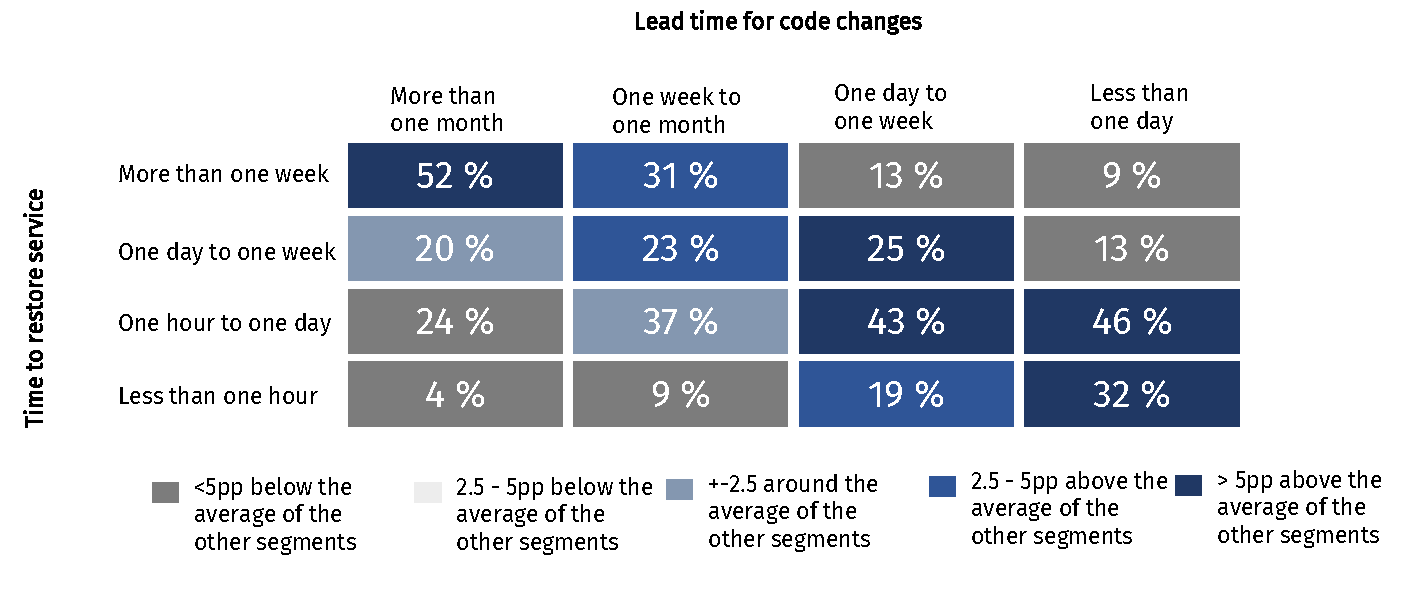
\includegraphics{Error}}
		\caption[Korrelation von Vorlaufzeit und Fehlerrate bei der Bereitstellung]{Korrelation von Vorlaufzeit und Fehlerrate bei der Bereitstellung. In Anlehnung an Berry.}
		\label{tab:Error}
	\end{table}
\end{center}
\vspace*{-15mm} 
Entschließt sich ein CE dazu Bereitstellungsprozesse zu automatisieren, sollte dieses strategisch dabei vorgehen. So empfiehlt Experte 5, Softwarearchitekt des SAP DTS, ein schrittweises Implementieren der Pipeline. Dabei sollte zunächst Erfahrung mit der Automatisierung einfacher isolierter Prozesse gesammelt werden \cite[Z. 8 ff.]{SoftwareArchitektSAPDTSIntegration.}. Anschließend können verbleibende, zur Bereitstellung von Software benötigten Schritte, in einem kontrollierten Tempo in die Pipeline eingebunden werden. Bei der Einführung von CI/CD ist ebenso entscheidend, dass Unternehmen spezifische Anforderungen abdeckende Tools verwenden. Dafür wurde im Rahmen dieser Arbeit ein Entscheidungs-Framework entworfen. Mit diesem wurde evaluiert, welches Pipeline-Tool zur Automatisierung der CI/CD-Prozesse für CEA den größten Mehrwert birgt. Unter Berücksichtigung der in Kapitel \ref{sec:Bewertung} abgewickelten Analyse, kann Azure Pipelines als das optimale CI/CD-Tool angesehen werden. Aus diesem Kontext lassen sich für dieses Pipeline-Tool einige Vorteile ableiten. Azure Pipelines unterstützt die Programmbibliothek Project Piper, mit welcher essenzielle Schritte für das Bauen, Testen und Bereitstellen von SAP-CAP-Node- und SAP-UI5-Anwendungen ausgeliefert werden. Die Bereitstellung vorimplementierter Schritte stellt sicher, dass sämtliche Compliance-Standards der SAP, wie Sicherheits- und Datenschutzbestimmungen, Branchenvorschriften oder interne Richtlinien, während des Bereitstellungsprozesses eingehalten werden. Obwohl die vorliegende Arbeit zur Beratung externer Kunden konzipiert ist, welche nicht verpflichtet sind, diese Richtlinien einzuhalten, sind diese oft in kritischen Sektoren, wie der Finanz- oder Versicherungsindustrie, tätig, bei welchen ebenfalls strikte Regularien gelten. Durch die Bereitstellung dieser standardisierten Bibliothek entfällt für Unternehmensentwickler somit die Notwendigkeit einer zeitaufwendigen Implementierung dieser Schritte. Neben der Möglichkeit, dass CEs auf diese Weise in der Lage sind, neue Services schnell bereitzustellen, erleichtert eine zentrale Bibliothek ebenfalls Aktualisierung und Pflege einzelner Pipeline-Schritte. Des Weiteren werden durch die Programmbibliothek Project Piper ebenfalls umfassende Bereitstellungsfunktionalitäten zur Verfügung gestellt. So umfasst diese neben vorimplementierten Schritten zum Ausrollen von Anwendungen auf der SAP BTP, ebenfalls ein Blue/Green-Deployment. Das Blue-Green-Deployment stellt eine effektive Möglichkeit dar, Software unter Produktionsbedingungen zu testen und kritische Ausfallszeiten bei der Bereitstellung von Software zu vermeiden. Dies spielt insbesondere dann eine wichtige Rolle, wenn Fehler in einem Microservice eines ERP-Systems auftreten, jedoch das herkömmliche Bereitstellen einer neuen Anwendungsversion aufgrund der durch die Initalisierung bedingten Ausfallzeit, zu unflexibel ist. Ein weiteres in Azure Pipelines kompatibles Bereitstellungskonzept ist das Multi-Cloud-Deployment. Damit können einzelne Module, wie CRM- oder SCM-Komponenten, auf unterschiedlichen Cloud-Plattformen ausgerollt werden. Neben einer Bereitstellung auf etablierten Cloud-Plattformen wie Google Cloud oder Amazon Web Services ermöglicht Azure Pipelines in diesem Kontext ebenfalls eine nahtlose Integration mit den eigenen Cloud-Diensten. Dieser Integrationsvorteil erstreckt sich ebenfalls auf andere Services, welche innerhalb des Azure-Ökosystems bereitgestellt werden. So umfasst dieses darüber hinaus Dienste, wie eine Entwicklungsumgebung, ein Projektmanagement- und Monitoring-Tool sowie ein Artefakt-Repository, welche mit geringem Aufwand in die CI/CD-Pipeline integriert werden können. Laut Experte 5 stellt Technologieoffenheit einen wichtigen Aspekt für CEs dar \cite[Z. 8 ff.]{SoftwareArchitektSAPDTSIntegration.}. Obwohl die Evaluation dieser Arbeit auf SAP-Technologien beschränkt ist, besteht die Möglichkeit, dass sich ein CEs dazu entscheidet einzelne Services auf anderen Programmiersprachen aufzubauen. Azure Pipelines stellt im Standard bereits unzählige Build-Tools sowie Test-Frameworks zur Verfügung. Sollte dieser jedoch nicht ausreichend sein, können mit Azure Pipelines ebenfalls Docker-Container aufgebaut werden. Mit diesen besteht die Möglichkeit Abhängigkeiten, wie Softwaretreiber, in einer isolierten Infrastruktur zu installieren, ohne von der Laufzeitumgebung der Pipeline abhängig zu sein. Azure Pipelines kann darüber hinaus zur Vereinfachung des Entwicklungsprozesses beitragen. So ist es Entwicklern möglich, Tests der Integration-Pipeline unmittelbar aus der Visual-Studio-Code-Umgebung auszuführen, ohne, dass Features zunächst in das Repository geladen werden müssen. Des Weiteren können mit dem CI/CD-Tool Pipeline-Implementationen sowohl lokal aus den Entwicklungsumgebungen, als auch zentral in dem Azure-Dashboard bearbeitet werden. Diese Praktikabilität ergibt sich ebenfalls bei der Ausführung der CI/CD-Pipelines. Im Falle von Fehlschlägen einzelner Schritte, besteht die Möglichkeit, dass nur fehlerhafte Schritte erneut ausgeführt werden. Auf diese Weise lassen sich bei temporären Problemen oder externen Abhängigkeiten, wie Ausfällen von Drittanbietern, Zeit und Rechenressourcen einsparen. Laut Experte 3 spielt dies insbesondere bei der Bereitstellung umfangreicher ERP-Services eine wichtige Rolle, da Pipeline-Schritte wie Code-Analysen mit unter über fünf Stunden in Anspruch nehmen können \cite[Z. 20 ff.]{ProductManagerSAPHyperspaceSecurityTools.}. Dies erwies sich ebenfalls im One-Strike Programm als einen bedeutenden Aspekt. In diesem Zusammenhang hat die SAP Maßnahmen ergriffen, um die Anzahl der Cloud-Provider, von welchen Dienste bezogen werden, zu reduzieren. Im Rahmen dieser Konsolidierung wurden Frontend-End-Pipelines für das S/4HANA-Core, welche zuvor auf Jenkins gehostet wurden, zu Azure migriert. Ein weiterer wesentlicher Aspekt für diesen Wechsel, waren Kostenüberlegungen. Durch die Nutzung einer SaaS-basierten CI/CD-Lösung können erhebliche Einsparungen bei Aufwandspositionen, Hardwareinvestitionen oder Wartungs- und Support-Kosten erzielt werden. Dieser Aspekt birgt insbesondere einen erheblichen Mehrwert für die CEA. Da Unternehmen mit dieser Architektur bestrebt sind, schnell auf disruptive Marktveränderungen zu reagieren, müssen diese in der Lage sein, Services wie CI/CD-Pipelines schnell auf- und abbauen bzw. skalieren zu können. Während in einem On-Premise-Modell hierfür ggf. hohe Investitionen erforderlich sind, werden Rechenressourcen bei Azure unmittelbar bereitgestellt und in Abhängigkeit der Nutzung bepreist (\textit{Pay-as-you-go}). Da die Bereitstellung von Services zum Kerngeschäft von Microsoft gehört, wird kontinuierlich in die Aktualisierung und Verbesserung der Azure-Infrastruktur investiert. Neben der Verwendung neuester Hardware wird die hohe Leistungsfähigkeit von Azure Pipelines ebenfalls durch das Bereitstellen von Optimierungsmechanismen sichergestellt. Dazu gehört etwa das parallele Ausführen verschiedener Pipeline-Schritte, was insbesondere bei umfangreichen Testvorgängen einen hohen Mehrwert birgt. Ferner besteht die Möglichkeit der Verwendung von Caching-Mechanismen. Damit können Ressourcen, wie Artefakte oder Daten, welche während des Pipeline-Prozesses heruntergeladen werden, für weitere CI/CD-Workflows  auf der Cloud zwischengespeichert werden. Laut Experte 4, haben diese Konzepte dazu beitragen, dass der CI/CD-Prozess der internen Standardentwicklung um 35 Prozent beschleunigt wurde \cite[Z. 58 ff.]{TestDeveloperSAPHyperspaceAdoption&Onboarding.}. Obwohl Azure Pipelines die für eine CEA essenziellen Funktionalitäten bereitstellt, besteht die Möglichkeit, dass Unternehmen aufgrund situativer Gegebenheiten, Jenkins oder SAP CI/CD verwenden. Dafür ausschlaggebende Gründe werden in dem in Abb. \ref{fig:Entscheidungsbaum} dargestellten Entscheidungsbaum aufgeführt.
Laut Experte 1 sollte SAP CI/CD insbesondere von Kunden verwendet werden, welche über wenige Microservices verfügen und somit keine komplexen Anforderungen an den Bereitstellungsprozess besitzen \cite[Z. 58 ff.]{ProductOwnerSAPBTPProd&Infra.}. Auch wenn mit SAP CI/CD für SAP CAP Node sowie SAP UI5 essenzielle Pipeline-Schritte bereitgestellt werden, sind Unternehmen mit diesem Tool in ihren Funktionalitäten eingeschränkt. Dies ist maßgeblich darauf zurückzuführen, dass das CI/CD-Tool ausschließlich eine Konfiguration und keine Implementierung der Pipelines zulässt. 
Laut Experte 1 ist dieses Tool jedoch insbesondere für Kunden vorgesehen, welche aus der traditionellen On-Premise-Umgebung auf die SAP BTP umsteigen \cite[Z. 58 ff.]{ProductOwnerSAPBTPProd&Infra.}. Hierbei besitzen Entwicklungs-Teams i.d.R. nicht über erforderliche DevOps-Kenntnisse, da diese zunächst mit dem Lernen allgemeiner Cloud-Konzepte, wie z.B. Programmier-Frameworks, beschäftigt sind. So soll das im Jahr 2020 veröffentlichte Tool kontinuierlich erweitert werden, um den wachsenden Anforderungen der Nutzer gerecht zu werden. 
\begin{center}
	\begin{figure}[H]\hspace*{-5mm}\hspace*{-11mm}
		\centering
		\scalebox{0.5}{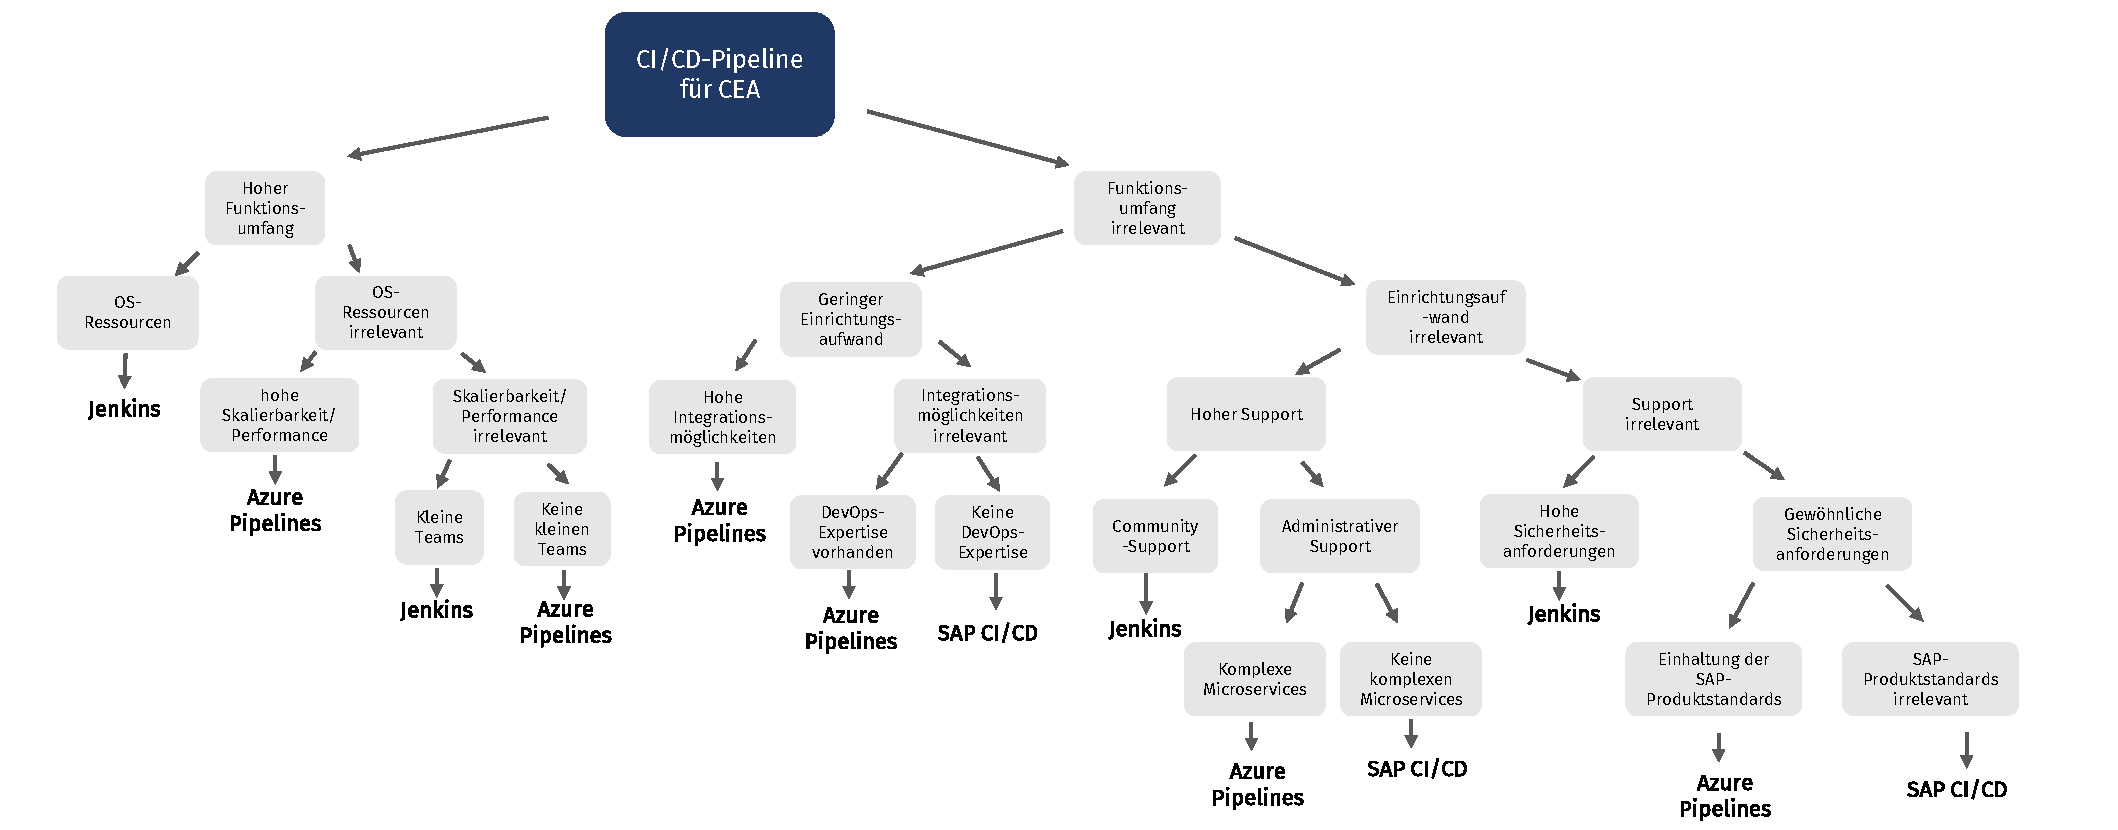
\includegraphics{Entscheidungsbaum}}
		\caption[Entscheidungsbaum für die Wahl eines CI/CD-Pipeline-Tools]{Entscheidungsbaum für die Wahl eines CI/CD-Pipeline-Tools. Eigene Darstellung.}
		\label{fig:Entscheidungsbaum}
	\end{figure}
\end{center}
\vspace*{-15mm}
Weiterhin empfiehlt sich dieses Tool für CEs, welche bereits ein umfangreiches Produktportfolio der SAP beziehen und auch zukünftig auf SAP-Technologien setzen möchten. So könnten SAP-Kunden, welche neben SAP CI/CD ebenfalls andere Services des Unternehmens beziehen, potenziell von niedrigeren Gebühren für das Tool profitieren. Eine weitaus höhere Flexibilität ergibt sich durch die Verwendung von Jenkins. Da dieses CI/CD-Tool On-Premise bereitgestellt wird, besitzt ein Unternehmen volle Kontrolle über die Gestaltung des Pipeline-Tools und kann dieses somit auf die Bedürfnisse der eigenen System-Architektur ausrichten. Dies ermöglicht eine flexible Anpassung der Infrastruktur-Komponenten, wie Server- und Netzwerkmodule, Sicherheitsprotokolle oder dem Datenmanagement. Somit bietet sich eine On-Premise-Pipeline insbesondere in Branchen an, in welchen Datensicherheit und Compliance-Anforderungen hohe Priorität besitzen. Dazu gehören etwa Finanzdienstleistungsinstitute, das Gesundheitswesen oder die öffentliche Verwaltung. Ein weiterer Grund für die Verwendung von Jenkins besteht darin, von den im Standard bereitgestellten Funktionalitäten unabhängig zu sein. Durch den Open-Source-Charakter des Tools, stehen den Entwicklern zahlreiche externe Ressourcen zur Verfügung. Dies können etwa von der Community entwickelte Plug-ins darstellen, welche in das Pipeline-System integriert werden können. Darüber hinaus haben DevOps-Spezialisten Zugang auf eine Vielzahl in Internet-Foren veröffentlichte Informationen. Dies unterstützt Entwickler dabei, Expertise, welche zur Implementierung einer maßgeschneiderten Pipeline benötigt wird, zu erlangen. Experte 4 bemerkt, dass Jenkins ausschließlich von kleinen Entwicklungsteams, welche mit einer geringen Anzahl an Technologien arbeiten, verwendet werden sollte \cite[Z. 58 ff.]{TestDeveloperSAPHyperspaceAdoption&Onboarding.}. Dies lässt sich darauf zurückführen, dass durch eine Aktualisierung diverse Plug-ins mit der neuen Jenkins-Version inkompatibel sein könnten. Folglich tendieren große Entwicklungsprojekte, welche eine Vielzahl heterogener Plug-ins verwenden dazu, eine Aktualisierung möglichst lange hinauszuzögern. Somit sollte darauf geachtet werden, dass dieses Pipeline-System ausschließlich in kleinen Entwicklungsprojekten mit wenig Abhängigkeiten verwendet wird.  
